%slide relative ad introdurre gli elementi di XML

% prendere da libro XML in amazon e XML visual quick view
% inserire qualche nota sul namespace anche preso dal libro xsd da pag 26 
% riprendere qualche slide dall slide Del Turco; e dalle slide Fiormonte-Ciotti-Silvi-XML-corso-2014.pdf
% http://filologiadigitale-verona.it/wp-content/uploads/2014/10/Fiormonte-Ciotti-Silvi-XML-corso-2014.pdf
% Slide Chiara di Pietro

% IDE/Editor Management Studio comes with a nice XML/XSD editor. It has a number of features that makes schema writing lot easier. Intellisense, auto-completion, real-time syntax checks, etc., are a few of those features.

\begin{frame}
	\frametitle{Fondamenti XML}
	\framesubtitle{eXtensible Markup Language}
	\addtocounter{nframe}{1}

	\begin{block}{XXXXXXXXXXXX}
		XML has its roots in Standard Generalized Markup Language (SGML), a language
		introduced in the 1980s that describes the structure and content of any machine-
		readable information.
	\end{block}

	\begin{block} {XXXXXXXXXXXXXXXXx}
		XML can be
		thought of as a lightweight version of SGML. Like SGML, XML is a language used to create vocabularies for other markup languages

	\end{block}
\end{frame}

\begin{frame}
	\frametitle{Fondamenti XML}
	\framesubtitle{eXtensible Markup Language}
	\addtocounter{nframe}{1}

	\begin{block}{XXXXXXXXXXXXXXXX}
		It is a set of rules for defining custom-built markup languages
	\end{block}

	\begin{block} {XXXXXXXXXXXXXXXXXX}

		XML was originally created to structure, store, and transport information.
		Like SGML,XML can be used to create XML applications or vocabularies, which are markup
		languages tailored to contain specific pieces of information.

	\end{block}
\end{frame}


\begin{frame}
	\frametitle{Fondamenti XML}
	\framesubtitle{eXtensible Markup Language}
	\addtocounter{nframe}{1}

	\begin{block}{XXXXXXXXXXXXXXXX}
		XML is a markup language that is extensible, so it can be m­odified
		to match the needs of the document author and the data being recorded
	\end{block}

	\begin{block} {XXXXXXXXXXXXXXXXXX}

		developed and maintained by the World Wide Web Consortium (W3C),
		an organization created in 1994 to develop common protocols and standards for
		sharing information on the World Wide Web

	\end{block}
\end{frame}

\begin{frame}
	\frametitle{Fondamenti XML}
	\framesubtitle{eXtensible Markup Language}
	\addtocounter{nframe}{1}

	\begin{block}{XXXXXXXXXXXXXXXX}
		XML, or eXtensible Markup Language, is a
		specification for storing information. It is also
		a specification for describing the structure of
		that information. And while XML is a markup
		language (just like HTML), XML has no tags
		of its own
	\end{block}

\end{frame}


\begin{frame}
	\frametitle{Fondamenti XML}
	\framesubtitle{eXtensible Markup Language}
	\addtocounter{nframe}{1}

	\begin{center}
		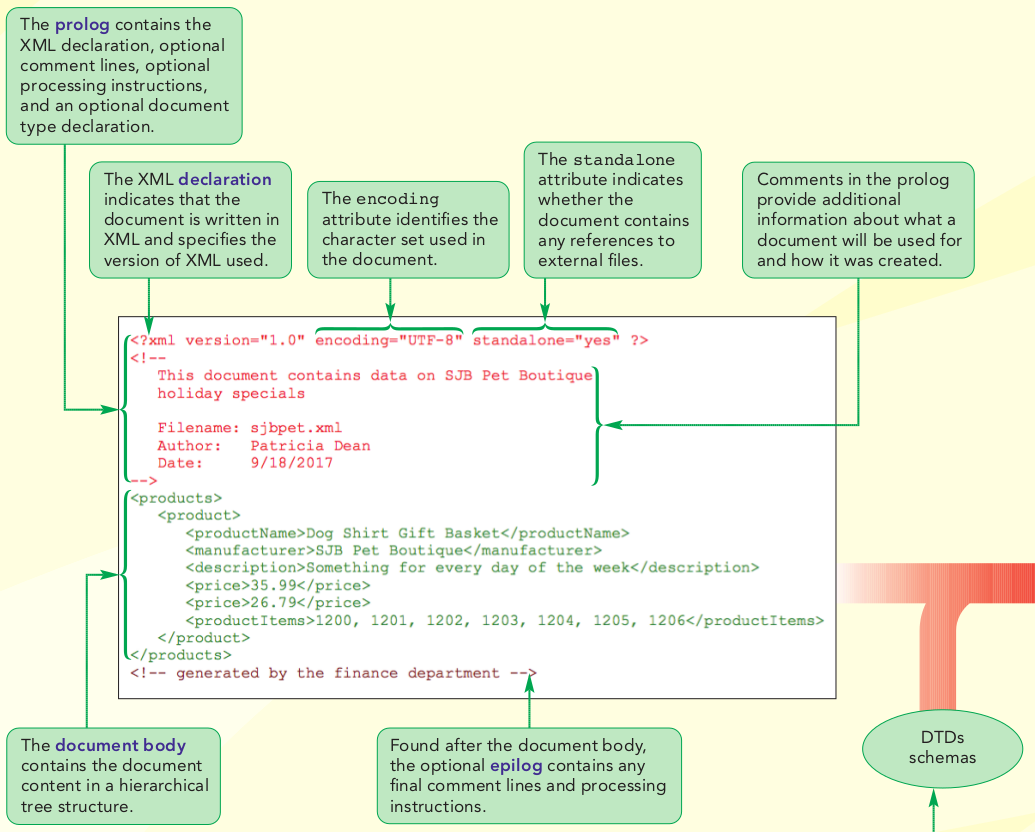
\includegraphics[width=.8\textwidth]{imgs/intro-doc-xml.png}
	\end{center}

	\begin{tiny}\textit{immagine dal libro New Perspectives on XML, 3rd Edition}\end{tiny}

\end{frame}


%The syntax rules of XML are easy to learn and easy to use
\begin{frame}
	\frametitle{Fondamenti XML}
	\framesubtitle{eXtensible Markup Language: Syntax Rules}
	\addtocounter{nframe}{1}

	\begin{itemize}

		\item Every XML element must have a closing tag.
		      %	Every element must have a closing tag. A self-closing tag is permitted.

		\item XML tags are case sensitive.
		      %   Opening and closing tags (or start and end tags) must be ­written with the same case.

		\item XML elements must be ­properly nested.
		      %All elements can have child (sub) elements. Child elements must be in pairs and be correctly nested within their respective parent element.

		\item Every XML document must have a root element.
		      %Every XML document must contain a single tag pair that defines	the root element. All other elements must be nested within the root element.

		\item XML elements can have attributes in name-value pairs.
		      %Each attribute name within the same element can occur only once.% Each attribute value must be quoted.

		\item Some characters have a ­special meaning in XML.
		      %The use of certain characters is restricted. If these characters are needed, entity references or character references may be used. References always begin with the character “&” (which is ­specially reserved) and end with the character “;”.

		      %XML allows for comments. 
		\item Comments cannot occur prior to the XML Declaration. Comments cannot be nested.

	\end{itemize}

\end{frame}


\begin{frame}
	\frametitle{Fondamenti XML}
	\framesubtitle{eXtensible Markup Language}
	\addtocounter{nframe}{1}

	\begin{block}{XML vista ad albero}
		XML is based on hierarchical trees in which order is significant.
		In XML, hierarchy and sequence are the main methods used to represent information.
	\end{block}

\end{frame}

\begin{frame}
	\frametitle{Fondamenti XML}
	\framesubtitle{eXtensible Markup Language}
	\addtocounter{nframe}{1}

	\begin{center}
		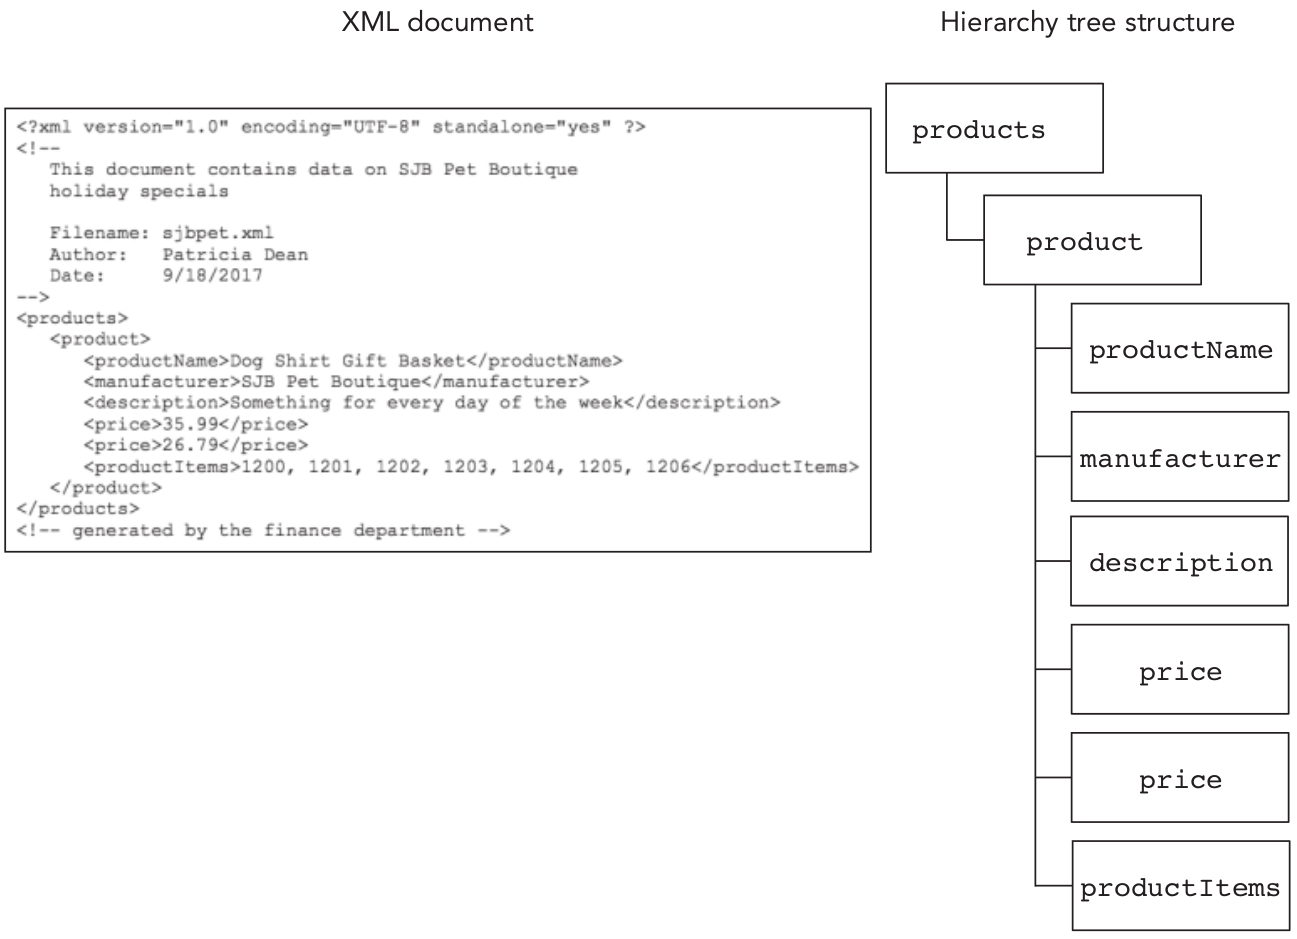
\includegraphics[width=.9\textwidth]{imgs/XML-TreeStructure.png}
	\end{center}

\begin{tiny}\textit{immagine dal libro New Perspectives on XML, 3rd Edition}\end{tiny}

\end{frame}

\begin{frame}
	\frametitle{Fondamenti XML}
	\framesubtitle{eXtensible Markup Language}
	\addtocounter{nframe}{1}

	\begin{block}{TEI-XML vocabulary}
		To meet the need of textual scholars, an XML ­vocabulary called Text Encoding Initiative (TEI) was developed, which codes text i­nformation.
	\end{block}

	\begin{block}{XML Vocabularies}
		XML vocabularies:  set of XML tags for a particular business function.
	\end{block}

\end{frame}


\begin{frame}
	\frametitle{Fondamenti XML}
	\framesubtitle{eXtensible Markup Language: Esempio TEI}
	\addtocounter{nframe}{1}

	\begin{center}
		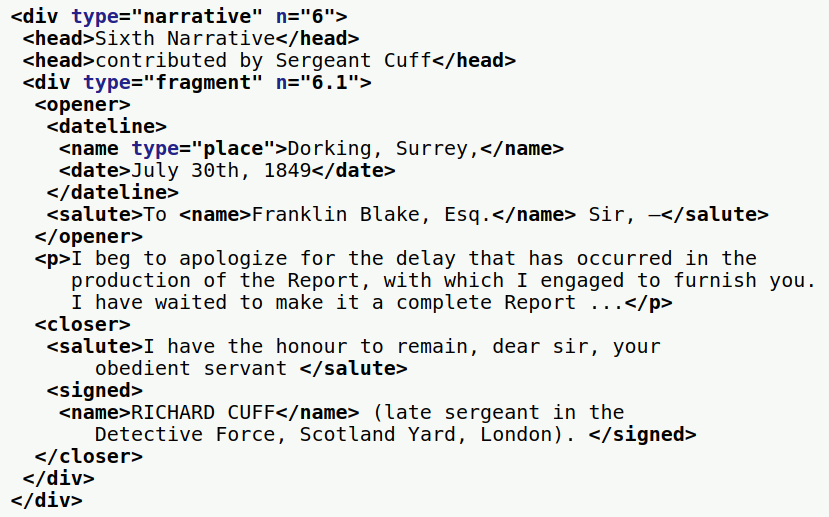
\includegraphics[width=.9\textwidth]{imgs/TEI-Example.png}
	\end{center}

	\begin{tiny}
        \textit{immagine dal sito TEI Guide Lines}
    \end{tiny}

\end{frame}

\begin{frame}
	\frametitle{Fondamenti XML}
	\framesubtitle{eXtensible Markup Language}
	\addtocounter{nframe}{1}

	\begin{block}{Manutenibilità}
		Because XML focuses on communicating the data, the overall structure is simple and easy to design and
maintain.
	\end{block}

\end{frame}

\begin{frame}
	\frametitle{Fondamenti XML}
	\framesubtitle{eXtensible Markup Language}
	\addtocounter{nframe}{1}

	\begin{block}{Documento ben formato (well-formed)}
        A well-formed document contains no syntax errors and satisfies the general specifications for XML code as laid
        out by the W3C. At a minimum, an XML document must be well formed or it will not
        be readable by programs that process XML code.
	\end{block}

\end{frame}


\begin{frame}
	\frametitle{Fondamenti XML}
	\framesubtitle{eXtensible Markup Language}
	\addtocounter{nframe}{1}

	\begin{block}{Parti principali di un documento XML}
        An XML document consists of three parts—the prolog, the document body, and the
        epilog. 
	\end{block}

\end{frame}


\begin{frame}
	\frametitle{Fondamenti XML}
	\framesubtitle{eXtensible Markup Language: Esempio TEI}
	\addtocounter{nframe}{1}

	\begin{center}
		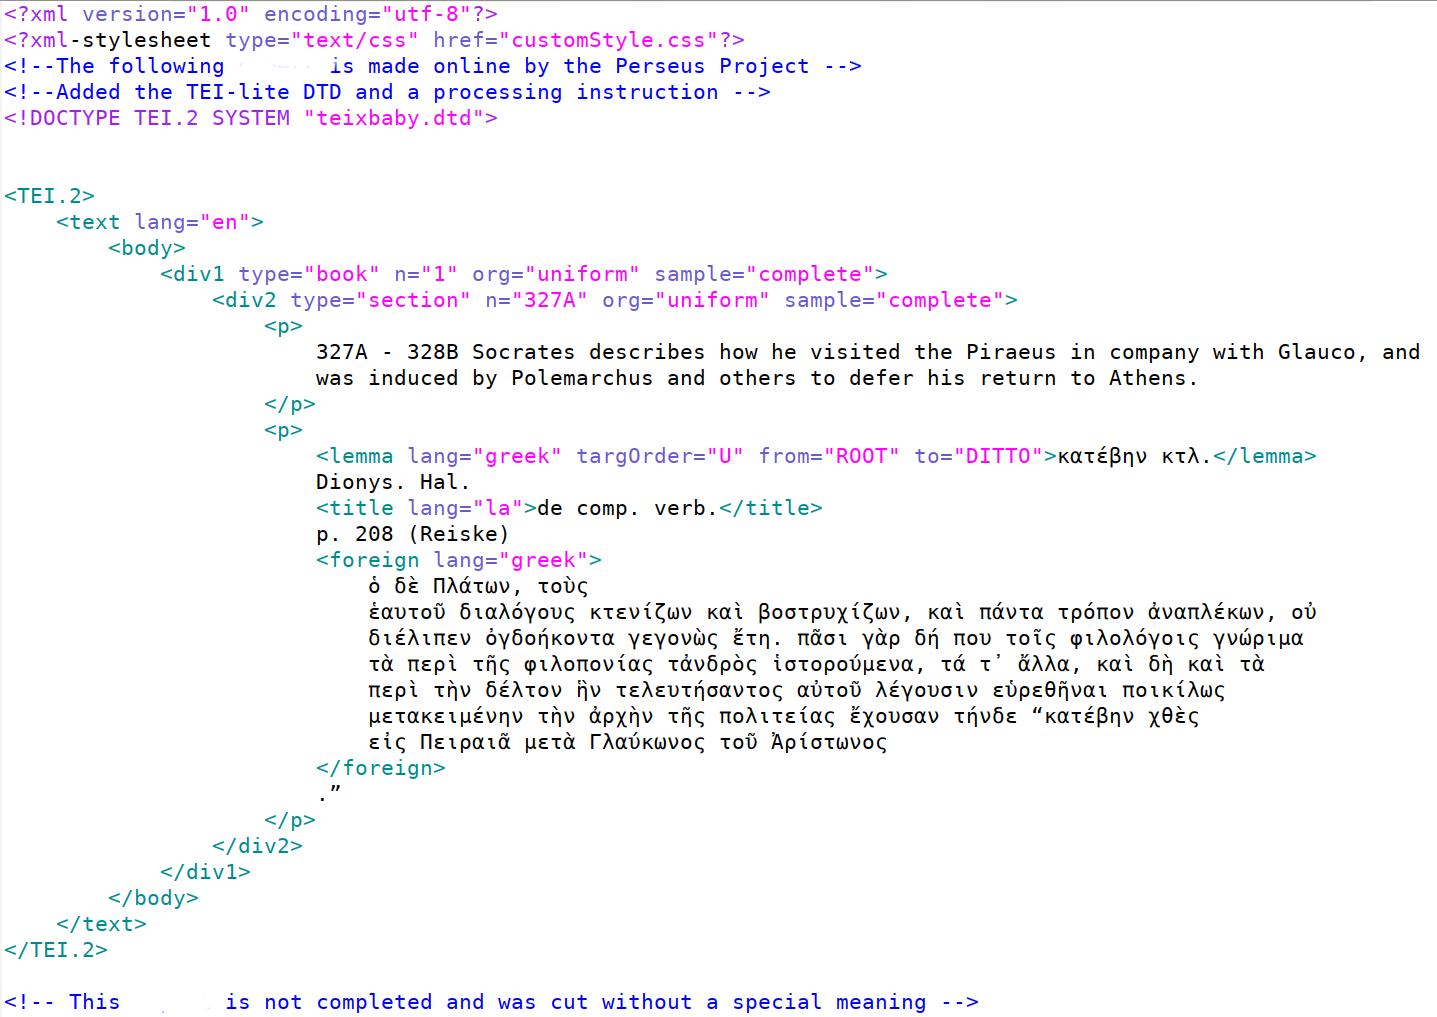
\includegraphics[width=1.1\textwidth]{imgs/TEI-PerseusExample.png}
	\end{center}

\end{frame}


\begin{frame}
	\frametitle{Fondamenti XML}
	\framesubtitle{eXtensible Markup Language}
	\addtocounter{nframe}{1}

	\begin{block}{Parti principali di un documento XML}
        The prolog includes the following parts:
        
        • XML declaration: indicates that the document is written in the XML language
        • Processing instructions (optional): provide additional instructions to be run by
        programs that read the XML document
        • Comment lines (optional): provide additional information about the document
        contents
        • Document type declaration (DTD) (optional): provides information about the rules
        used in the XML document’s vocabulary
	\end{block}

\end{frame}

\begin{frame}
	\frametitle{Fondamenti XML}
	\framesubtitle{eXtensible Markup Language}
	\addtocounter{nframe}{1}

	\begin{block}{Parti principali di un documento XML}
        The document body, found immediately after the prolog, contains the document’s
        content in a hierarchical tree structure. Following the document body is an optional
        e­pilog, which contains any final comments or processing instructions.
	\end{block}

\end{frame}

\begin{frame}
	\frametitle{Fondamenti XML}
	\framesubtitle{eXtensible Markup Language: Prologo}
	\addtocounter{nframe}{1}

	\begin{block}{XML declaration}
    \begin{center}\texttt{<?xml version=”version number” encoding=”encoding type” standalone=”yes|no” ?>}\end{center}
	\end{block}

\end{frame}

Creating an XML Declaration
• To create an XML declaration, enter the code
<?xml ?>
in the first line of an XML document.
• To specify a version of XML to use, enter the code
version=”version number”
after the opening <?xml tag, where version number is either 1.0 or 1.1.
• To specify a character encoding, enter the code
encoding=”encoding type”
after the version attribute-value pair, where encoding type identifies the ­character
set used in the document.
• To indicate whether the document is a standalone document, enter the code
standalone=”yes|no”
after the encoding attribute-value pair, where the value yes or no ­indicates whether
access to external files will be needed when processing the document.


ERRORI:
<?XML VERSION=”1.0” ENCODING=”ISO-8859-1” STANDALONE=”YES” ?>
<?xml version=1.0 encoding=ISO-8859-1 standalone=yes ?>
<?xml version=”1.0” standalone=”yes” encoding=”ISO-8859-1” ?>

Generally speaking, comments are ignored by programs reading the document and
do not affect the document’s contents or structure.
To insert a comment in an XML document, enter
<!-- comment -->

If you have a comment that will occupy more than one line, you can
continue the ­comment on as many lines as you need


ESERCIZIO

<!--
This document contains data on SJB Pet Boutique
holiday specials
Filename: project.xml
Author:
your name
Date:
today's date
-->


A program that reads and interprets an XML document is called an XML processor or XML parser, or simply a processor or parser.

First well-formed
A second function of a parser is to interpret PCDATA in a document and resolve any character or
entity references found within the document
finally, an XML document might contain
processing instructions that tell a parser exactly how the document should be read and
interpreted

The current versions of all major web browsers include an XML parser of some type.

To test for well-formedness, you’ll use an XML parser to compare the XML document against the
rules established by the W3C.
INTRODURRE XMLLINT


The document body in an XML document is made up of elements that contain data

to be stored in the document. Elements are the basic building blocks of XML files.

An ­element can have text content and child element content.

<element>content</element>
The opening tag is <element> , and </element> is the closing
tag.

▪ Gli elementi XML possono avere diversi tipi di contenuto:
▫ contenuto strutturale: solo altri elementi, non testo
▫ contenuto misto: testo e anche altri elementi
▫ contenuto testuale: solo testo, non altri elementi

Element names might be established already if an author is using a particular XML
vocabulary, such as TEI-XML


There are a few important points to remember about XML elements:
• Element names are case sensitive, which means that, for example, itemnumber,
itemNumber, and ItemNumber are unique elements.
• Element names must begin with a letter or the underscore character ( _ ) and may not
contain blank spaces. Thus, you cannot name an element Item Number , but you can
name it Item_Number .
• Element names cannot begin with the string xml because that group of ­characters is
reserved for special XML commands.
• The name in an element’s closing tag must exactly match the name in the ­opening tag.
• Element names can be used more than once, so the element names can mean
different things at different points in the hierarchy of an XML document.

Creating XML Elements
XML 24
• To create an XML element, use the syntax
<element>content</element>
where element is the name given to the element, content represents the text
content of the element, <element> is the opening tag, and <
­ /element> is the
closing tag.
• To create an empty XML element with a single tag, use the following syntax:
<element />
• To create an empty XML element with a pair of tags, use the syntax
<element></element>


An open element or empty element is an element
with no content.

<element />
where element is the name of the empty element

<element></element>
a two-sided tag with no content


Empty
elements can also contain attributes that can be used to store ­information

Nesting Elements
In addition to text content, elements also can contain other elements.
An element
contained within another element is said to be a nested element.

ESEMPIO
<product>
<productName>Dog Shirt Gift Basket</productName>
<manufacturer>SJB Pet Boutique</manufacturer>
<description>Something for every day of the week</description>
<price>35.99</price>
<price>26.79</price>
<productItems>1200, 1201, 1202, 1203, 1204, 1205, 1206
</productItems>
</product>

hierarchical relationships between
elements
A nested element is a child element of the element in which it is nested—
its parent element
Elements that are side-by-side in a document’s ­hierarchy are
sibling ­elements

syntax error in creating an XML document is improperly nesting

XML does not allow the opening and ­closing
tags of parent and child elements to overlap

Esercizio: scrivere e fare il check di un xml non opportunamente annidato

The Element Hierarchy
All elements in the body are children of a single element called the
root element or document element.

hierarchy represented in a tree diagram

Note that the XML declaration and comments are not included
in the tree structure of the document body

An XML document must include a root element to be considered well formed

However, by indenting the code and placing siblings on their own lines, you can visually
reveal the hierarchy relationships and add a dimension of visual communication to your
code.

A quick way to view the overall structure of a document body is to chart the ­elements
in a tree structure

It would be useful to have a general tree diagram that indicates whether a particular
child element can occur zero times, once, or several times within a parent

The symbols ?, *, and + are part of the code used in creating DTDs to validate XML
documents.

MIXED CONTENT
Mixed content elements are ideal for
descriptive, text-based chunks of infor-
mation. They are not very common in
database-type applications.

In some cases, you may want an element to
contain both content and child elements.
This is referred to as mixed content

ESEMPIO
<wonder>
Temple of Artemis at Ephesus
<city>Ephesus</city>
<country>Turkey</country>
</wonder>

Esercizio:
aprire il file XML non ben formato nella cartella xml e:
- correggerlo (mettendo come commenti la correzione fatta e brevente spiegarla)
-- nested, case sensitive
- aggiungere un figlio (child) all'elemento XYZ1
- aggiungere un fratello (sibling) all'elemento XYZ2

Working with Attributes
Every element in an XML document can contain one or more attributes
An attribute
describes a feature or characteristic of an element

<element attribute=”value”> ... </element>
<element attribute=”value” />

Attribute values are text strings. Therefore, an attribute value always must be enclosed
within either single or double quotes.

Esempio:
(preso dalla TEI)

name for an attribute as long as it meets the following rules:
• An attribute name must begin with a letter or an underscore ( _ ).
• Spaces are not allowed in attribute names.
• Like an element name, an attribute name should not begin with the text string xml.

An attribute name can appear only once within an element. Like all other aspects of
XML, attribute names are case sensitive, and incorrect case is a common syntax error
found in attributes.
The order of attributes is not significant and there is no way to control the order of attributes

Adding an Attribute to an Element
• To add an attribute to an element, use the syntax
<element attribute=”value”> ... </element>
where element is the name given to the element, attribute is the ­attribute’s
name, and value is the attribute’s value.
• To add an attribute to a single-sided tag, use the syntax
<element attribute=”value” />
• To specify multiple attributes for a single element, use the syntax
<element attribute1=”value1” attribute2=”value2” ...> ... </element>
where attribute1 is the first attribute’s name, value1 is the first attribute’s value,
attribute2 is the second attribute’s name, value2 is the second ­attribute’s
value, and so on. Each attribute is separated by a space.

It’s not always clear when to use an attribute value rather than inserting a new element.
A general rule of thumb is that if all of the XML tags and their attributes were
removed from a document, the remaining text should comprise the document’s content
or information.
Another rule of thumb is that attributes should be used to describe data, but should
not contain data themselves.
Different developers have different preferences, and
there’s no right answer.

Using Character and Entity References
a numeric character reference, also known simply as a ­character
reference. The syntax for a character reference is
&#nnn;
where nnn is a character number from the ISO/IEC character set

the character numbers for different symbols,
some symbols also can be identified using a character entity reference—also known
si­mply as an entity reference—using the syntax
Unicode can be used in
conjunction with entity
references to display
specific characters or
symbols.
&entity;

Immagine


Inserting Character and Entity References
• To insert a character reference into an XML document, use
&#nnn;
where nnn is a character reference number from the ISO/IEC character set.
• To insert an entity reference, use
&entity;
where entity is a recognized entity name.


text characters fall into three categories—parsed
character data, character data, and white space.


Parsed Character Data
Parsed character data (PCDATA) consists of all those characters that XML treats as parts
of the code of an XML document.
• the XML declaration
• the opening and closing tags of an element
• empty element tags
• character or entity references
• comments

The presence of PCDATA can cause unexpected errors to occur within a document
This means that symbols such as &, <, or >, which are all used in ­creating
markup tags or entity references, are extracted and the appropriate content is used in your
program.

Character Data
Character data is not processed,
but instead is treated as pure data content.

As an alternative to using character references, you can place text into a CDATA section.
A CDATA section is a block of text that XML treats as character data only. The syntax for
creating a CDATA section is
<![CDATA [
		character data
	]]>

In a
CDATA section, these characters are interpreted by XML parsers or XML editors as text
rather than as markup commands. A CDATA section
• may be placed anywhere within a document.
• cannot be nested within other CDATA sections.
• cannot be empty.

The only sequence of symbols that may not occur within a CDATA section is ]]
because this is the marker ending a CDATA section.

Esempio:
The following example shows an element named htmlCode containing a CDATA
section used to store several HTML tags:
<htmlCode>
<![CDATA[
		<h1>SJB Pet Boutique</h1>
		<h2>Fashion for Pets and Their Humans</h2>
	]]>
</htmlCode>

You can use CDATA blocks when you want to include large blocks of special
characters as character data

You cannot use XML comments in a CDATA section.

You cannot nest a CDATA section inside another CDATA section

White Space

White space refers to nonprintable characters such as spaces, new lines, tabs.
Technically, no white space ­stripping
occurs for element content, which means that the content of the XML element

When white space appears in places other than element content, XML treats it in the
following manner:
• White space is ignored when it is the only character data between element tags; this
allows XML authors to format their documents to be readable without affecting the
content or structure.
• White space is ignored within a document’s prolog and epilog, and within any
element tags.
• White space within an attribute value is treated as part of the attribute value.

Esercizio:
inserire attributi e CDATA section


Inserting a Processing Instruction
A processing instruction is a command that tells an XML parser how to process the
document.
<?target instruction ?>

where target identifies the program (or object) to which the processing instruction is
directed and instruction is information that the document passes on to the parser for
processing.

Usually the instruction takes the form of attributes and attribute values

Esempio:
<?xml-stylesheet type=”text/css” href=”main.css” media=”all” ?>
Multiple processing instructions can exist within the same XML document for different
media types

Working with Namespaces
A namespace is a defined collection of element and attribute names.
An XML vocabulary could define a single namespace.

involves two steps:
1. Declare the namespace.
2. Identify the elements and attributes within the document that belong to that
namespace.

Add an attribute
within the opening tag for the element using the syntax
<element xmlns:prefix=”uri”> ... </element>

(URI)—a text string that uniquely identifies a resource.
The purpose of a URI is simply to provide a
unique string of characters that identify a resource.
One version of a URI is the Uniform Resource Locator (URL)
URLs serve as a built-in mechanism on the web for generating unique addresses
Note that although a URI
doesn’t actually need to point to a real site on the web, it’s often helpful to place
documentation at the site identified by a URI so users can go there to learn more
about the XML vocabulary being referenced.

Esempio TEI ns.

In addition, a namespace that has been declared within an element can
be applied to any descendant of the element.

The number of namespace attributes that can be declared within an element is
unlimited.

root element so that each namespace is available to all
elements within the document

You can declare a default namespace by omitting the prefix in the namespace ­declaration.
Any descendant element or attribute is then considered part of this namespace unless a
different namespace is declared within one of the child elements.


<element xmlns=”uri”> ... </element>

Esempio TEI


Declaring a Namespace
• To declare a namespace for an element within an XML document, add the
xmlns:prefix attribute to the opening tag of the element using the syntax
<element xmlns:prefix=”uri”> ... </element>
where element is the element in which the namespace is declared, prefix is the
namespace prefix, and uri is the URI of the namespace.
• To declare a default namespace, add the xmlns attribute without specifying a prefix,
as follows:
<element xmlns=”uri”> ... </element>

% XML document is primarily composed of elements and attributes
% Attributes can only exist within an element. An attribute declaration really does not make sense without an element.
% Attributes can only store a value, while elements can also store child elements and attributes.
% An element can appear more than once within a parent node, but an attribute can appear only once. The order of attributes is not significant and there is no way to control the order of attributes in XSD. If the attribute is present the default value is not assigned, even if the value of the attribute is an empty string.
% the default value of elements is assigned only when the element is present and is empty
% Elements are mandatory by default while attributes are optional by default.


%Both HTML and XML use tags in similar ways, often creating distinctly hierarchical structures to present data to users.

% Like HTML documents, XML documents can be created and viewed with a basic text editor such as Notepad or TextEdit. More sophisticated XML editors are available, and using them can make it easier to design and test documents.


% slide su XML lint


% tanti vocabolari XML
% Bioinformatic Sequence Markup
% Language (BSML) Coding of bioinformatic data
% Extensible Hypertext Markup Language
% (XHTML) HTML written as an XML application
% Mathematical Markup Language
% (MathML) Presentation and evaluation of mathematical equations
% and operations
% Music Markup Language (MML) Display and organization of music notation and lyrics
% Weather Observation Definition
% Format (OMF) Distribution of weather observation reports, forecasts, and
% advisories
% Really Simple Syndication (RSS) Distribution of news headlines and syndicated columns
% Synchronized Multimedia Integration
% Language (SMIL) Editing of interactive audiovisual presentations ­involving
% streaming audio, video, text, and any other media type
% Voice Extensible Markup Language
% (VoiceXML) Creation of audio dialogues that feature synthesized
% speech, digitized audio, and speech recognition
% Wireless Markup Language (WML) Coding of information for smaller-screened devices, such
% as PDAs and cell phones